%\documentclass[twocolumn,showpacs,prb,superscriptaddress,aps,floatfix]{revtex4-1}
\documentclass[preprint,showpacs,prb,superscriptaddress,aps,floatfix]{revtex4-1}
\usepackage{rotating}
\usepackage{amsmath}
\usepackage{color}
\usepackage{graphicx}
\usepackage{epsfig}
\usepackage{courier}
\usepackage[active]{srcltx}
\usepackage[sort&compress]{natbib}


\newcommand{\uu}{{\bf u}}
\newcommand{\qq}{{\bf q}}
\newcommand{\ab}{{\bf a}}
\newcommand{\bb}{{\bf b}}
\newcommand{\hh}{{\bf h}}
\newcommand{\rr}{{\bf r}}
\newcommand{\pp}{{\bf p}}
\newcommand{\PP}{{\bf P}}
\newcommand{\kk}{{\bf k}}
\newcommand{\HH}{{\bf H}}
\newcommand{\GG}{{\bf G}}
\newcommand{\SiS}{{\bf \Sigma}}
\newcommand{\VV}{{\bf V}}
\newcommand{\UU}{{\bf U}}
\newcommand{\w}{\omega}
\newcommand{\tf}{\textbf}
\newcommand{\bo}{\mathbf}
\newcommand{\br}{{\bf r}}
\newcommand{\be}{\begin{equation}}
\newcommand{\ee}{\end{equation}}
\newcommand{\ben}{\begin{equation*}}
\newcommand{\een}{\end{equation*}}
\newcommand{\bea}{\begin{eqnarray}}
\newcommand{\eea}{\end{eqnarray}}
\newcommand{\bean}{\begin{eqnarray*}}
\newcommand{\eean}{\end{eqnarray*}}
\newcommand{\nup}{n_{\uparrow}}
\newcommand{\ndown}{n_{\downarrow}}
\newcommand{\Id}[1] {\int \! \! {\rm d}^3 #1}
\renewcommand{\v}[1]{{\bf #1}}
\renewcommand{\[}{\left[}
\renewcommand{\]}{\right]}
\renewcommand{\(}{\left(}
\renewcommand{\)}{\right)}
\def\efield{\boldsymbol{\cal E}} 
\def\ket#1{\vert#1\rangle}
\def\bra#1{\langle#1\vert}



 
\newcommand{\grenoble}{Institut N\'eel,
CNRS/UJF, 25 rue des Martyrs BP 166, B\^{a}timent D 38042 Grenoble
cedex 9 France} 
\newcommand{\rome}{Istituto di Struttura della Materia (ISM), Consiglio Nazionale delle Ricerche, Via Salaria Km 29.5, CP 10, 00016 Monterotondo Stazione, Italy}
\newcommand{\coimbra}{Centre for Computational Physics and Physics Department, University of Coimbra, Rua Larga, 3004-516 Coimbra, Portugal}

\begin{document}
\title{Simple model for high-harmonic generation}
\author{C. Attaccalite}
\affiliation{\grenoble}

\begin{abstract}
In these notes I consider a simple tight-binding model in Wannier guage and write down the equation of motion of the density matrix in such a way to study its non-linear response and in particular the high-harmonic generation. I discuss all steps for the implementation in a computational code. 
\end{abstract}           

\maketitle

\section{Unit cell and atomic positions}
As simple system I consider a two-dimensional hexagonal boron nitride as shown in Fig.~\ref{fig:hbn_lattice}. 
\begin{figure}
  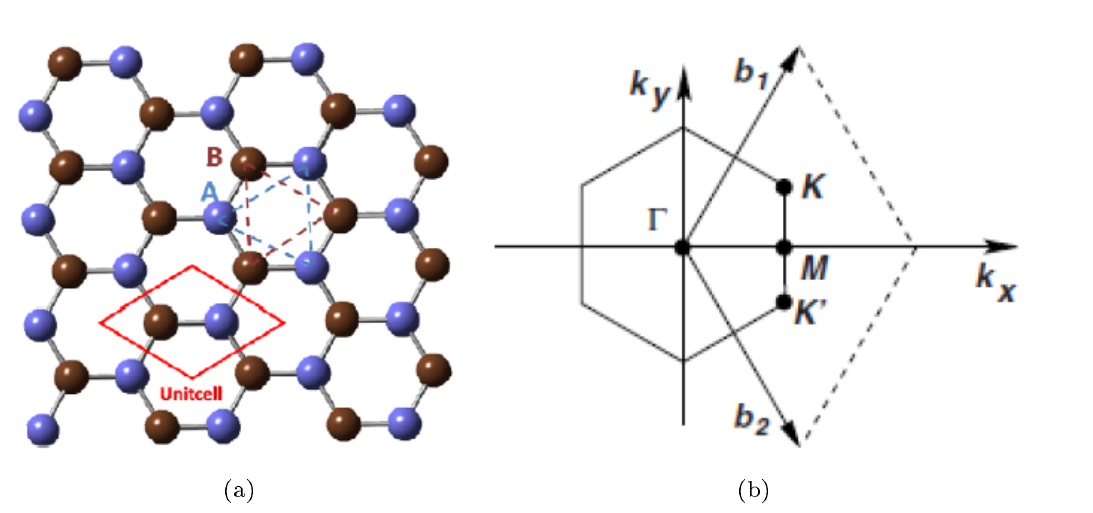
\includegraphics[width=\linewidth]{hbn.png}
  \caption{Hexagonal BN direct and reciprocal lattice.}
  \label{fig:hbn_lattice}
\end{figure}
Lattice vectors are defined as\footnote{I always define quantities in 3D for pratical implementation in the code}:
\bea
a_1&=&\frac{a}{2}\left ( 3, \sqrt{3}, 0 \right)  \\
a_2&=&\frac{a}{2}\left ( 3, -\sqrt{3}, 0 \right)  \\
a_3&=& \left( 0, 0, 1 \right)  \\
\eea
and the volume is $V=a_3 \cdot (a_1 \times a_2) = 3\sqrt{3} a^2/2$ 
and reciprocal lattice vectores are defined as:
\bea
b_1&=&\frac{2\pi}{V} a_2 \times a_3 = \frac{2\pi}{a} \left( 1,  \sqrt{3}, 0\right) \\
b_2&=&\frac{2\pi}{V} a_3 \times a_1 = \frac{2\pi}{a} \left( 1, -\sqrt{3}, 0\right) \\
b_3&=&\frac{2\pi}{V} a_2 \times a_3 = 2\pi \left( 0, 0, 1\right) \\
\eea

\section{Tight binding model}
\section{Wannier and Hamiltonian gauge}
\subsection{Gauge transformation}
\section{Position operator in periodic system}
\appendix
\section{Derivatives in k-space}
In general to perform derivative in k-space we define quantities as:
\be
\PP = \frac{1}{2\pi} \sum_{i=1,3} \ab_i (\PP \cdot \bb_i) = \frac{1}{2\pi} \sum_{i=1,3} \ab_i \PP_i
\ee
where $\bb_i$ are reciprocal lattice vectors and $\ab_i$ direct lattice vectors that satisfy the relation:
\be
\ab_i \cdot \bb_j = 2\pi\delta_{ij}
\ee
then the derivative along a $\bb_i$ vector can be rewritten in cartesian coordinates as:
\be
\nabla \PP = \frac{1}{2\pi} \sum_{i=1,3} \ab_i \left( \frac{\partial \PP_i}{\partial \kk_i} \right)
\ee 
where $\kk_i$ are k-points along the $\bb_i$ vector.

\addcontentsline{toc}{chapter}{Bibliography}
\bibliographystyle{apsrev4-1}
\bibliography{hhg}
\end{document}
